\documentclass{beamer}

\usepackage[utf8]{inputenc}
\usepackage{graphicx}
\usepackage{xmpmulti}

\usepackage{tikz}
\usetikzlibrary{positioning}

\setbeamertemplate{navigation symbols}{}

\title{News from the SoundScape Renderer}
\subtitle{\url{http://spatialaudio.net/ssr/}}
\author{Matthias Geier}
\institute{}
\date{Lightning Talk\\June 9, 2018\\Linux Audio Conference, Berlin}


\begin{document}
\maketitle

{
\setbeamertemplate{background canvas}
[vertical shading][top=white,middle=structure.fg!40,bottom=white]
\setbeamertemplate{background}{%
\begin{tikzpicture}[remember picture, overlay]
\node[anchor=north east,yshift=-0.5cm] at (current page.north east)
{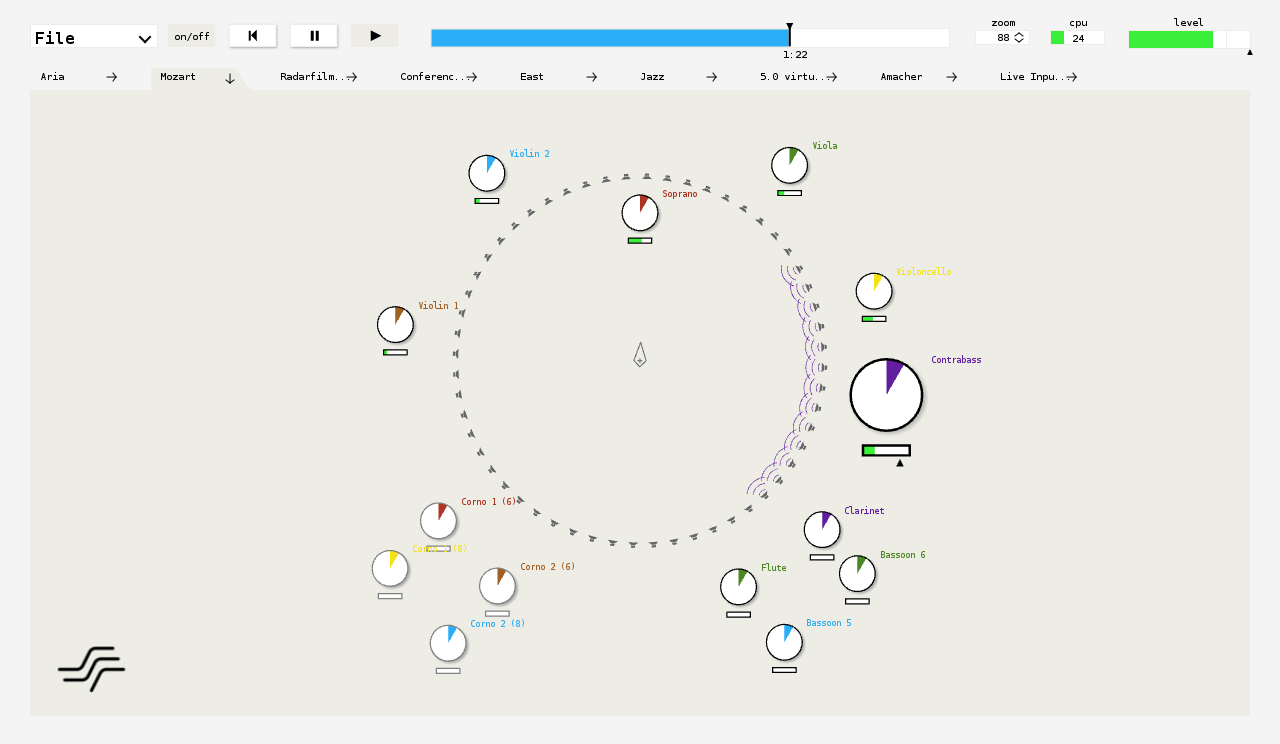
\includegraphics[scale=.27]{img/mozart_full_muted_wfs}};
\node[anchor=south west] at (current page.south west)
{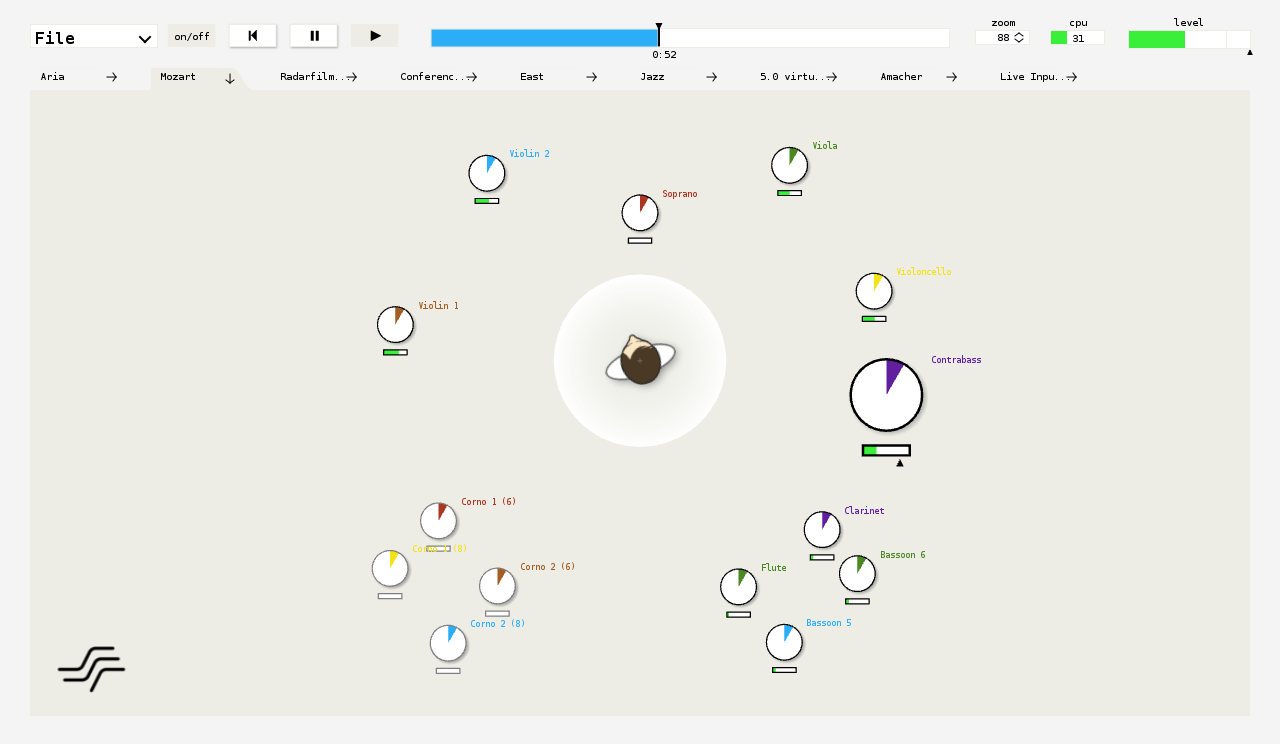
\includegraphics[scale=.27]{img/mozart_full_muted_binaural}};
\end{tikzpicture}
}
\setbeamertemplate{footline}{}
\begin{frame}
\frametitle{\hspace{-.3333em}\tikz[baseline=(x.base)] \node[fill=white,fill opacity=.6,text opacity=1,text depth=0pt] (x) {SoundScape Renderer (SSR)};}
%\framesubtitle{Graphical User Interface}
% no frame text
\end{frame}
}

\begin{frame}{SoundScape Renderer (SSR)}
\begin{itemize}
%\item software tool for \emph{scene-based} realtime spatial audio reproduction
\item several different reproduction methods
\begin{itemize}
\item Binaural Renderer
\item Binaural Room Synthesis (BRS)
\item Wave Field Synthesis (WFS)
\item NFC-HOA Renderer (it's broken, though \dots)
\item Vector Base Amplitude Panning (VBAP)
\item Ambisonic Amplitude Panning (AAP)
\item Generic Renderer
\end{itemize}
\end{itemize}

\pause

\begin{itemize}
\item runs on Linux and Mac OS X (limited support for Windows)
\item uses the \emph{Jack Audio Connection Kit} (JACK)
\item graphical user interface (Qt) and network interface (TCP/IP)
\item Free and Open Source Software (GPLv3)
\item \url{http://spatialaudio.net/ssr/}
\end{itemize}
\end{frame}

\begin{frame}{SSR as a Library}
\begin{itemize}
\item renderers can be easily used in any C++ program
\begin{itemize}
\item with multi-threading
\end{itemize}
\item only audio processing
\begin{itemize}
\item no JACK
\item no GUI
\item no network
\item no scene files
\end{itemize}
\item \dots\ as real-time plugin
\begin{itemize}
\item e.g. PureData external
\end{itemize}
\item \dots\ for offline processing
\begin{itemize}
\item e.g. MEX file for Octave/Matlab
\end{itemize}
\end{itemize}
\end{frame}

\begin{frame}%{PureData External}
\begin{center}
\multiinclude[<visible@+>][format=png,graphics={scale=0.7}]{img/pd-screenshot}
\end{center}
\end{frame}

\begin{frame}{Current Limitations, Future Work}
\begin{itemize}
\item extend to 3D
\item dynamic scenes
\item more network interfaces: WebSockets, OSC, \dots?
\item move to browser-based GUI (using WebGL)
\item Python wrapper
\item Pure Data package (Deken)?
\item full Windows port?
\end{itemize}
\end{frame}

\begin{frame}
\begin{center}
Thanks for your attention!
\vfill
\url{http://spatialaudio.net/ssr/}
\vfill
\end{center}
\end{frame}

\end{document}
